
%(BEGIN_QUESTION)
% Copyright 2010, Tony R. Kuphaldt, released under the Creative Commons Attribution License (v 1.0)
% This means you may do almost anything with this work of mine, so long as you give me proper credit

Suppose a differential pressure transmitter is used to measure the pressure dropped across a {\it baghouse}, an assembly using multiple fabric ``socks'' to filter particulate material from a gas stream, like a large-scale vacuum cleaner.  Gas passes through the socks, filtering out the particulate matter.  The DP transmitter's pressure measurement serves to indicate how clogged the socks are:

$$\includegraphics[width=15.5cm]{i00021x01.eps}$$

When the transmitter signal reaches a certain value (indicating clogged filter socks), a control system triggers either a mechanical shaker or a blast of gas from jets located near each sock shakes the dust from the outside area of each sock, the dust falling down into the narrow area below where it is extracted over time from the baghouse.

\vskip 10pt

Suppose an instrument technician leaves the three valves in the positions shown (hollow = open ; solid = closed).  What effect will this have on the socks over time as they perform their filtering job, assuming the control system continues to operate as designed?

\vfil

\underbar{file i00021}
\eject
%(END_QUESTION)





%(BEGIN_ANSWER)

This is a graded question -- no answers or hints given!

%(END_ANSWER)





%(BEGIN_NOTES)

With the block valves shut and the equalizing valve open, the control system ``thinks'' there is no pressure drop across the socks, and therefore {\it never} triggers the mechanism(s) to shake dust loose from the bags.  As a result, the bags will clog with dust and the baghouse will eventually plug up.

%INDEX% Measurement, pressure: troubleshooting
%INDEX% Process: baghouse filter (generic)

%(END_NOTES)


